\documentclass[12pt,a4paper,english,magyar,oneside]{report}
\usepackage[T1]{fontenc}
\usepackage[utf8]{inputenc} % mert nem a középkorban vagyunk
\usepackage{indentfirst} % fejezetek első bekezdését is húzzuk be
\usepackage{lmodern} %szépek lesznek tőle a betűk a pdfben
\usepackage{graphicx}
\usepackage{amsmath}
\usepackage{float}
\usepackage{wrapfig}
\usepackage{tcolorbox}
\usepackage{lipsum}

\usepackage[magyar]{babel}

% 2.5 centis margó mindenütt, bal oldalt +1 centi kötésnek
\usepackage{anysize}
\paperwidth=21cm \paperheight29.7cm
\marginsize{3.5cm}{2.5cm}{2.5cm}{2.5cm} % {bal}{jobb}{felső}{alsó}
\addtolength\topmargin{-\headheight} \addtolength\topmargin{-\headsep}
\addtolength\textheight{\headheight} \addtolength\textheight{\headsep}
\addtolength\textheight{\footskip}
\footskip=15pt
\ifx\pdfoutput\UnDefined \newcount\pdfoutput \fi
\ifnum0<\pdfoutput
  \pdfpagewidth\paperwidth \pdfpageheight\paperheight \pdfcompresslevel9
\else \special{papersize=21cm,29.7cm} \fi

\sloppy % inkább a térköz nőljön minthogy sorok lógjanak ki jobb szélen

\linespread{1.3} % Másfeles sorköz
\frenchspacing   %Szimpla térköz mondatok között

\begin{document}

\begin{center}

\begin{figure}[!h]
  \begin{center}
    \resizebox{8.5cm}{!}{
    \includegraphics{fig/BMEkicsi2.jpg}
        }
  \end{center}
\end{figure}

Budapest University of Technology and Economics \\
Faculty of Electrical Engineering and Informatics\\
{\small Department of Automation and Applied Informatics}

\thispagestyle{empty}

\pagestyle{empty}

\vspace{3.5cm}

\Large Attila Fodor

\vspace{0.8cm}

\textbf{\uppercase{\LARGE Autonóm felszíni oceanográf}}

% Úgy tűnik az \uppercase nem szereti az ékezetes betűket :(

\vfill

\textsc{Consultant:}\\ \Large Kundra László

\vspace{0.6cm}

\normalsize Budapest, \today

\end{center}

\clearpage

%--------------------------------------------------------

\iffalse

\chapter*{\uppercase{Hallgatói nyilatkozat}}

\thispagestyle{empty}

Alulírott, Fodor Attila szigorló hallgató kijelentem, hogy ezt a diplomatervet meg nem engedett segítség nélkül, saját magam készítettem, csak a megadott forrásokat (szakirodalom, eszközök, stb.) használtam fel. Minden olyan részt, melyet szó szerint, vagy azonos értelemben, de átfogalmazva más forrásból átvettem, egyértelműen, a forrás megadásával megjelöltem.

Hozzájárulok, hogy a jelen munkám alapadatait (szerző(k), cím, angol és magyar nyelvű tartalmi kivonat, készítés éve, konzulens(ek) neve) a BME VIK nyilvánosan hozzáférhető elektronikus formában, a munka teljes szövegét pedig az egyetem belső hálózatán keresztül (vagy autentikált felhasználók számára) közzétegye. Kijelentem, hogy a benyújtott munka és annak elektronikus verziója megegyezik. A teljes szöveg közzététele dékáni engedéllyel titkosított diplomatervekre nem vonatkozik.


\vspace{5 cm}

\begin{tabular}[h]{c c c}

Kelt: Budapest, \today & \hspace{2cm} & \rule{5cm}{.4pt} \\

 & & Fodor Attila

\end{tabular}

\clearpage

\setlength{\parindent}{0.2cm}
\fi %fedlap

\selectlanguage{english}

\chapter*{Abstract}

Abstract goes here.

\selectlanguage{magyar}

\chapter*{Kivonat}

A kivonat ide kerül.

\selectlanguage{english}

\setcounter{tocdepth}{2} % tartalomjegyzék mélysége
\tableofcontents % tartalomjegyzék

%\chapter*{Introduction}\addcontentsline{toc}{chapter}{Introduction}
\section{Introduction}

Seaborne measurements are often expensive and time consuming, though they can have a large impact on the area, where the data have been obtained. In 2011 the naval safe zone around the Fukusima accident was laid down based only on estimates of the radiation contamination\cite{FNPP}, because low amount of measurement data was available due to high measurement costs and risks. Another notable example are the coastal waters of Greenland, because are very poorly mapped up to present day\cite{2009AGUFMOS21A1152W}. Ships have to sail in a roundabout way around the island, because the risk of wrecking in unknown fjordic area is very high. This is a huge waste of time and natural resources annually.

\subsection*{Oceanography and Bathymetry}

Not many people come across these expressions often. Oceanography can be summarized as a branch of Earth science that studies the ocean. It includes a wide range of topics, like the study of marine ecosystem, ocean currents, plate tectonics and the geology of the sea floor. Bathymetry is the study of underwater depth of lake or ocean floors. The advancing technology allows even more possibilities, like the aforementioned radiological measurements, or general monitoring of the seas.

\subsection*{Advantages of autonomous vessels}

Oceanographic measurements today are carried out by large crewed ships, but in many cases they could be replaced by a number of smaller crafts, in order to reduce surveying time and cost and increase the available manpower in other tasks. These vessels could have the ability to sail previously unsurveyable areas as well, thanks to the shallower draught and smaller size.

\subsection*{Limitations}

The most notable limitation of the current mobile robotic technologies are their small size itself. It means the relatively small range based on their smaller power capabilities, and narrow field of application.

The aim of this project is to develop an autonomous surface vehicle, which is capable of conducting multiple seaborne measurements. To execute an oceanography mission, the ship must be capable of autonomus navigation based on Global Positioning System (GPS) and an Internal Measurement Unit (IMU), to further enhance the precision in hazardous environment.

\begin{figure}[H]
	\centering
	\includegraphics[width=0.8\textwidth]{img/aauship}
	\caption{The AAUSHIP prototype on her maiden voyage}
	\label{fig:aauship}
\end{figure}

\subsection*{Development guidelines}
In order to keep a sensible and extendable system, the control software of the ship follows the guidelines of the Model-Based Design approach. The system software can be divided to two different kind of modules, one that is dependent, and one that is independent from the physical characteristics of the vessel. In order to maximize the extendability of the system, the fix (independent) modules must be completely general, but as thorough as possible, so as to keep the complexity of the changeable (dependent) software of the robot minimal.
\begin{wrapfigure}{r}{0.48\textwidth}
  \begin{center}
    \includegraphics[width=0.5\textwidth]{img/trieste}
  \end{center}
  \caption{Bathyscaphe Trieste, the first manned vessel that reached the bottom of Challenger Deep (Mariana Trench)\cite{trieste}}
\end{wrapfigure}

The environment stored in the control system must be extendable to the third dimension, and must be able to track changes over time.
The tasks of the low level control must be as specific and as basic as possible. All calculations and control should be implemented in the high level controller.
the high level controller must be parametrized, based on the low level and hardware characteristics.

The point of these guidelines is to create a system of components with major reusability. Ideally a general Cross-platform High Level Controller controls different kind of vessels, through a standard interface. When changing to an arbitrary different vehicle, only the Low Level Controller must be replaced, which stores the characteristics of the vessel and implements the actuator control.

\section*{Operation models}

 A typical oceanography application starts on the shore. A science team analyzes the currently available data, then marks the area of measurements on the map. The  map data is transformed to a measurement path by the scientists or by the automatic waypoint planner of the ship. The autonomous surface vehicle is then outfitted with the right sensors for the task, and a manned ship transports it close to its destination. The crew can set the research vessel to manual, automatic or fully autonomous mode.

\paragraph{Manual control}
In this mode it's possible for the operator to control the movement of the ship, degree of freedom-wise or control the actuators themselves. The primary intent of this mode is for testing or malfunction-recovery.

\begin{figure}[H]
	\centering
	\includegraphics[width=0.8\textwidth]{img/manualcontrol}
	\caption{Manual remote control}
	\label{fig:manualcontrol}
\end{figure}

\paragraph{Automatic control}
In automatic mode the "brains", remain on the crewed vessel, and the research craft remains in wireless connection with the Mothership. When the measurements are complete, the oceanographer returns to the mothership. In automatic mode it is always possible to switch to manual control and back, or update the measurement path, etc.

\begin{figure}[H]
	\centering
	\includegraphics[width=0.8\textwidth]{img/automatic}
	\caption{Automatic supervised control}
	\label{fig:automatic}
\end{figure}

\paragraph{Autonomus control}
In Autonomus mode the ship carries everything that is needed to complete the task. Connection to the mothership can be cut, and the vessel carries the orders out autonomusly. Intervention in this mode is only possible until the oceanographer is in range of the mothership.

\begin{figure}[H]
	\centering
	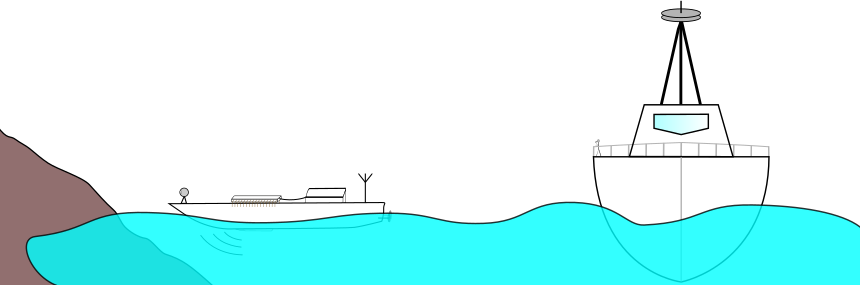
\includegraphics[width=0.8\textwidth]{img/autonomus}
	\caption{Autonomus control}
	\label{fig:autonomus}
\end{figure}

\paragraph{Squadron mode}
In case there are multiple research vessels, they can form a squadron. In this setup only one of the ships needs to be in range of the crewed mothership. Alternatively one autonomus ship is capable of controlling multiple automatic crafts, taking over the role of the mothership.

\begin{figure}[H]
	\centering
	\includegraphics[width=0.8\textwidth]{img/multiple}
	\caption{Squadron mode}
	\label{fig:multiple}
\end{figure}

\begin{tcolorbox}[colback=cyan!5,colframe=cyan!40!black,title=Code: Main.py \\ https://www.dropbox.com/s/h1067ywmdajkegk/Main.py]
\begin{minipage}{0,6\textwidth}
The mission planning steps are implemented in Main.py, which is the main part of the program, responsible for initializing the system, setting the target area, mode of routing, navigation, etc. Later Main.py will provide a Graphical User Interface as well.
\end{minipage}
\begin{minipage}{0,35\textwidth}
\raggedleft
\includegraphics[width=0.8\textwidth]{img/main}
\end{minipage}

\end{tcolorbox}

\section{Pathplanning} 

The first part of the document will lay down the basic concepts and requirements of an oceanography task, focusing on the development of the High Level Controller and a seamless simulator to evaluate the results.

\subsection{Map reading}

The main method of navigation is via GPS and known shoreline database. The ship must be outfitted with proximity sensors later, in order to ensure safe navigation through traffic. During the simulation a reference shore is being generated that simulates a typical fjordic environment: Figure~\ref{fig:linemap}. The map generator is using Random Walk Functions to generate the coastline(s).

\begin{figure}[H]
	\centering
	\includegraphics[width=0.8\textwidth]{img/linemap}
	\caption{The coastlines}
	\label{fig:linemap}
\end{figure}

The generated coastlines are converted to the actual Map, which is a number of surfaces: Figure~\ref{fig:solidmap}.

\begin{figure}[H]
	\centering
	\includegraphics[width=\textwidth]{img/solidmap}
	\caption{The solidified map (the picture shows a north ("upside down") coast)}
	\label{fig:solidmap}
\end{figure}

Reading a solid map is possible from image files as well, using the Python SciPy library

\begin{figure}[H]
	\centering
	\includegraphics[width=0.8\textwidth]{img/worldmap}
	\caption{Image file processed to Map object}
	\label{fig:worldmap}
\end{figure}

\section{Routing}

Upon entering the water, the first task of the vessel in automatic or autonomus mode is to determine the course. Currently the software can not handle rivers, strong wind and magnetic declination, therefore the course is assumed to be identical to the heading.

\paragraph{The Waypoint planner} is responsible for the generating and ordering of the key measurement points. Visiting a set of waypoints on a given map leads to the Traveling Salesman NP-complete problem. Even using dynamic programming, determining the best route with the Held-Karp algorithm the program requires $O(N^2 2^2)$ steps [wiki]. The problem has been in the crosshair of mathematics for a long time, but a fast exact solution has never been found. The waypoint-planning is not time-critical, but a sufficient length of path should be calculated in a reasonable amount of time.

Fortunately the arrangement of the measurement points is relatively dense and predictable, allows only neighboring travels and repeated visits. In order to reach a suitable algorithm, some heuristics of the path planning needs to be examined.
\\

\begin{tcolorbox}[colback=cyan!5,colframe=cyan!40!black,title=Code: Ship.py \\ https://www.dropbox.com/s/fmtsaatql7jqjhw/Ship\texttt{\_}nofilter.py]
\begin{minipage}{0,6\textwidth}
Ship.py implements the Ship Object. Everything related to the handling of a ship is encapsulated in a Ship instance. Multiple instances can be created based on the same object, with different parameters, and they are using the same resources.
\end{minipage}
\begin{minipage}{0,35\textwidth}
\raggedleft
\includegraphics[width=0.8\textwidth]{img/ship}
\end{minipage}
\end{tcolorbox}

\paragraph{In a simple coastline} the points can be placed in a certain order relative to the coast, to achieve a sufficient result. If the shore is relatively smooth, the ship can also travel parallel to the coast, to decrease the required number of turns.

\begin{figure}[H]
	\centering
	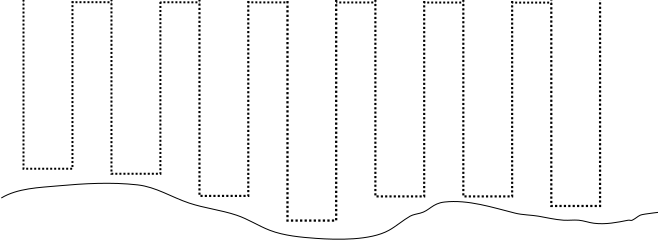
\includegraphics[width=\textwidth]{img/simplecoast}
	\caption{A simple coast and a sufficient path}
	\label{fig:simplecoast}
\end{figure}

\paragraph{Introducing isles and deep bays} to the area complicate the situation. Some waypoints need to be removed, and an avoiding path needs to be taken. This will cause many redundant measurements and very sub-optimal path, if the island density and the complexity of the coast is high.

\begin{figure}[H]
	\centering
	\includegraphics[width=\textwidth]{img/pathislands}
	\caption{Coast with islands}
	\label{fig:pathislands}
\end{figure}

\paragraph{Greedy traversal}

stretches a measurement grid over the area, and the points are traversed in an unpredictable way, using a neirest neighbourgh algorithm.

\begin{figure}[H]
	\centering
	\includegraphics[width=\textwidth]{img/traversal}
	\caption{A random path based on graph traversal}
	\label{fig:traversal}
\end{figure}

 According to [citation] heuristic closest neighbour search is usually 5-10\% worse than the ideal solution. Using the closest neighbour heuristic, the simulation leads to the following path: Figure~\ref{fig:nn}.

\begin{figure}[H]
	\centering
	\includegraphics[width=\textwidth]{img/nn}
	\caption{Neirest neighbourgh algorithm}
	\label{fig:nn}
\end{figure}

\subsection{Lowest cost heuristics}

Even without major nautical engineering skills the following presumption can be made: If there are two paths with identical start and finish and identical lengths (start != finish) the  path with less turning is more effective.
This presumption can be extended to the following theory:

The most effective nautical path between two given points is the one with the least sum cost. The sum cost is the traveled distance times distance cost, plus absolute turnining times turning cost.

\begin{align}
	\Sigma C  = dist*C_{dist} + |turn| * C_{turn}
\end{align}

The cost of the distance and the turning depends on the type of the ship. A large, deep draught cargo ship capable of low speed will have a much higher $\frac{Distance}{Turn}$ cost ratio than a narrow military cruiser.


Using the considerations above a cost based nearest neighbour algorithm is introduced, where the lowest distance is replaced with lowest cost. The algorithm checks every point to determine which is the cheapest destination. To avoid path-loops in the map, the waypoints already visited are stored in a list. If the examined point is already in the list, the cost is increased with a redundancy value, so the algorithm will chose a different, slightly more expensive, but still unvisited measurement point. The algorithm also checks, if the path leading to the examined waypoint is clear of obsticles.

Running the simulation with the above pathplanner results in the following course: Figure~\ref{fig:lc}.

\begin{figure}[H]
	\centering
	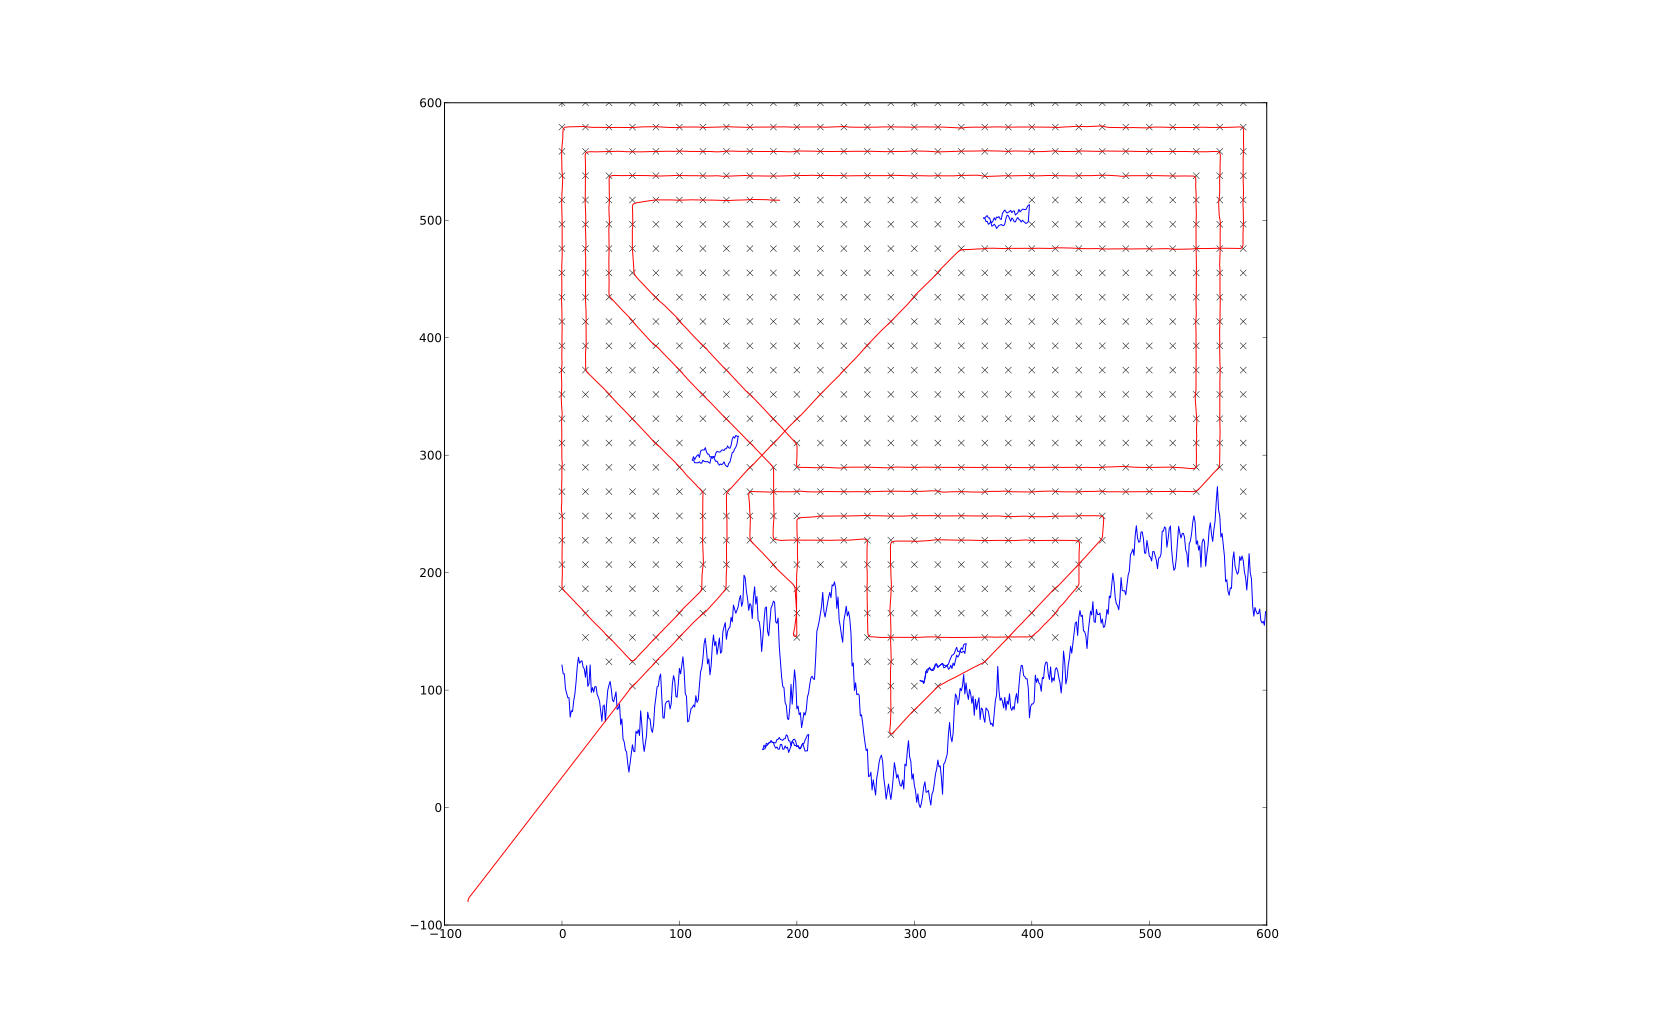
\includegraphics[width=\textwidth]{img/geee}
	\caption{Lowest cost algorithm}
	\label{fig:lc}
\end{figure}

This navigation method works adequatly in open environments. However, if the map is consisted of tight narrows and hard to navigate areas, the algorithm above fails to exit certain areas of the map. To be able to operate in such shores, a different kind of routing is required.

I call this method "Ripple", because the points examined are moving away from the surface vessel in a circular shape (well, in a rectangular actually) like a ripple. The ripple checks every neighbouroing waypoint, that wasnt checked so far, and stores the previous life of the ripple. If a point is found that has not been visited before, a list of waypoints are returned, and the ship will sail through them, and reach the destination.

Figure~\ref{fig:ripple} illustrates this navigation method by simulating a task on the map of the Earth.

\begin{figure}[H]
	\centering
	\includegraphics[width=\textwidth]{img/ripple}
	\caption{Ripple routing algorithm}
	\label{fig:ripple}
\end{figure}

\section{Navigation}

Once the required course has been set, the control system will take over the handling of the ship. The Navigation is the first and highest layer of control in the High Level Controller. In order to explain the navigation, the coordinate systems must be defined first.

\subsection{Frames of reference}

The operator team and the GPS sensor are using the Earth Centered Earth Fixed (ECEF) coordinate systems. Navigation on a spherical surface would introduce a lot of unnecessary calculations in every control cycle, since a plane can be fit onto the surface with minimal error, because the small vessel has limited maximum range.

During the Navigation the North East Down coordinate system is used to determine the attitude and position of the ship. The NED coordinate system is centered to the first GPS measurement coordinate.

A third Body Frame is also defined, the dynamic system of the ship was calculated in this frame.

\begin{figure}[H]
	\centering
	\includegraphics[width=\textwidth]{img/reference_frames}
	\caption{Used coordinate systems}
	\label{fig:coordinatesystem}
\end{figure}

\begin{align}
	\lambda = longitude  \quad \phi = latitude
	\\ GPS_{[\lambda , \phi , h]} \Longleftrightarrow [X_{NED}; Y_{NED}; Z_{NED}]
\end{align}

\subsection{Required heading}

The heading of the ship is defined in NED coordinate system. The required heading is determined by the Law of Cosines, based on the Position of the Ship and the Position of the next Sub-Waypoint.
\begin{center}
\includegraphics[scale = 0.4]{img/Law_of_Cosines}
\end{center}
Problems rise and corrections are necessary, if the heading of the ship $\theta$ is $\theta < -\pi$ or $\theta < \pi$. The heading of the ship is calculated based on the Gyro sensor and the heading can have any value in the form of: 
\begin{align}
\theta = [-{\pi} ; \pi ] \pm 2 \cdot k \cdot \pi
\end{align}\\

\begin{tcolorbox}[colback=cyan!5,colframe=cyan!40!black,title=Code: FunctionLibrary.py \\ https://www.dropbox.com/s/7nx7helisvss21a/FunctionLibrary.py]
\begin{minipage}{0,6\textwidth}
Some functions required by the software are general parametric mathematical functions, which can not be connected to any object. These functions, like the Law of Cosines, and the distance calculator function can be found in the Function Library.
\end{minipage}
\begin{minipage}{0,35\textwidth}
\raggedleft
\includegraphics[width=0.8\textwidth]{img/functionlibrary}
\end{minipage}


\end{tcolorbox}

Before invoking the control procedure, all of the heading angles must be transformed into the $[-\pi ; \pi]$ interval.
This procedure causes a possible error though.

\includegraphics[width=\textwidth]{img/Headings}

The required heading or the heading of the ship must be transformed into a different representation, where 
\begin{align}
|\theta_{r}-\theta| < \pi
\end{align}
To keep a consistent heading representation, first the deviation angle 
\begin{align}
\theta = \pi_{r}-\pi
\end{align} is calculated, than transformed to the $[-\pi;\pi]$ interval and finally, with $\delta$ we can transform $\theta_{r}$ to 
\begin{align}
\theta_{r}(\theta) = \theta + \delta
\end{align}
If the conditions above are met, $\theta$ and $\theta_r(\theta)$ will always yield values that result in correct controller output.

\section{Simulator}
In order to test the generated path and eliminate some hazards of potential design errors or malfunctions, a seamless simulator is required that simulates the behaviors of the ship. \\

\begin{tcolorbox}[colback=cyan!5,colframe=cyan!40!black,title=Code: Simulator.py \\ https://www.dropbox.com/s/agron9anslev6xw/Simulator.py]
\begin{minipage}{0,6\textwidth}
According to the guidelines of the seamless simulator, this part of the system has its own distinctive object. Everything related to the simulator and everything that is unknown during the mission is stored and handled here.
\end{minipage}
\begin{minipage}{0,35\textwidth}
\raggedleft
\includegraphics[width=0.8\textwidth]{img/simulatorcode}
\end{minipage}
\end{tcolorbox}

\subsection{Requirements of the simulator}

The simulator developed for the project must meet the following conditions, otherwise the simulation might return false results, misguiding the whole development process.
\begin{itemize}
	\item The software controlling the simulated system must be unaware of the simulation
	\item The control software must be completely independent of the simulator, its variables and its functions
	\item The control software can communicate only through the same channel, as it would during normal operation
	\item Any parameters and states that are not known, only measured (e.g.: measured position != actual position) must be stored in the simulator, and must not be accessed directly from the control software
\end{itemize}

To fulfill the requirements above, the following simulator has been implemented:

\begin{figure}[H]
	\centering
	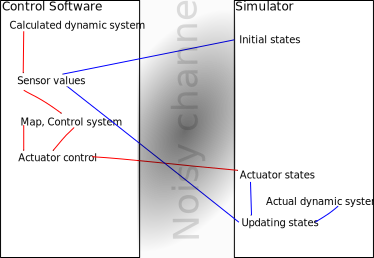
\includegraphics[width=\textwidth]{img/simulator}
	\caption{System simulator}
	\label{fig:simulator}
\end{figure}
\part{Project Laboratory II.}
\setcounter{section}{0}

It was shown in Part I. that the control software can fulfill its requirements, it's time to step forward and prepare the surveying platform: the BMESHIP.

\section{System overview}

This section will give a preliminary overview about the logical and physical layout of the system. The design steps were implemented using the guidelines of the Model Based Design approach, therefore the the logical layout resembles the physical. However, for a lighter approach, the layouts will be introduced separately and connected later.

\subsection{Logical layout}

This basic layout describes the logical connections of the system:

\begin{figure}[H]
	\centering
	\includegraphics[width=0.8\textwidth]{img2/LogicalLayout}
	\caption{The logical layout of the system}
	\label{fig:LogicalLayout}
\end{figure}

The High Level Interface (HLI) processes the position and orientation sensor data input from Bluetooth serial port. During regular navigation the HLI applies the filtering to the inputs, then outputs the estimated orientation divergence from the path, and the estimated distance from the path. The Controller (C) processes this data and returns the required inputs to the system. The LLI processes this physical signal and transforms them to PWM signals, then applies it to the power electronics and the Actuators (A), which will have the final effect on the system.

It’s important to note in this diagram, that the Controller and is separated from the rest of the software. This enables the user to radically modify the configuration of the robot, or try multiple controller implementations and switch between them real-time. The 
Such a switching system can handle possibly expected failures and breakdowns up to a certain level (like the malfunction of one of the engines of a twin-propeller aircraft).

\subsection{Physical layout}

The more detailed physical layout diagram shows the actual relations of the modules of the system to each other. There are several rapid prototyping technologies working together, all of them based on very high level languages.

The embedded system is running Angström Linux, which is a lightweight linux distribution. It enabled the use of Python and USB Hardware-extensions, a generic cheap USB Bluetooth Dongle and a webcam (The webcam is working, but it’s not supported yet on the software level).
Using Linux as the operating system of the embedded device has the additional advantage of manually controlling and updating the system through SSH.

The HLI and LLI are both implemented in Python. They communicate through function calls implemented via Cython. The actual Controller and Kalman Filter run natively, the .c/.h source code is compiled to .so files by the Cython compiler, which can be imported into the main python software as a static function library.

The source code files are generated by MATLAB Embedded Coder, based on the Simulink model of the control system. The resulting functions are more like objects, containing inner states and member functions, but only one instance can exist of the same controller object.

The GPIOs are controlled from Python as well, using system calls.

\begin{figure}[H]
	\centering
	\includegraphics[width=1\textwidth]{img2/PhysicalLayout}
	\caption{The physical layout of the system}
	\label{fig:PhysicalLayout}
\end{figure}

The Embedded system has an USB Bluetooth hardware extension that communicates with the GPS receiver and the Client software.
It’s important to note, that the GPS receiver and the Embedded system are physically close to each other (relative to the scale of the ship), always within the range of the Bluetooth connection. Using wireless communication however enables the distant placement (relative to the scale of the circuit board) in order to ensure high GPS reception and a protected environment for the embedded system as well (e.g.: top of the mast and the belly of the boat).

\subsection{Validation \& Verification}

V\& V has become a very popular concept recently, but has always been a vital process in the development of mission-critical systems. Losing or sinking the prototype due to faulty design or construction would have a devastating effect on my thesis, therefore I treated the system as mission-critical, trying to ensure very high reliability.

Validation requirements of the system:

\begin{itemize}

\item The robot can of navigate along a specified path
\item The robot can map a set of points in a given map
\item The robot can always find it’s way, if there exists any

\end{itemize}

Verification requirements of the control system:

\begin{itemize}

\item The controller can process sensor data into valid state readings
\item The controller ensures the asymptotic stability of the closed-loop system 

\end{itemize}

\begin{figure}[H]
	\centering
	\includegraphics[width=0.8\textwidth]{img2/SimVer}
	\caption{}
	\label{}
\end{figure}

Verification requirements of the communication:

\begin{itemize}

\item The system can transmit and receive serial Bluetooth data
\item The system can process the incoming data
\item The system can automatically re-establish connection with the slave Bluetooth devices (GPS and client)
\item The system shuts down after a time period if connection was lost

\end{itemize}

\subsection{Verification requirements of the client software}

\begin{itemize}

\item The system can transmit and receive serial Bluetooth data
\item The system can provide valid real-time information about the system
\item The system can automatically re-establish connection with the master Bluetooth device (HLI)

\end{itemize}

\begin{figure}[H]
	\centering
	\includegraphics[width=0.6\textwidth]{img2/VeriBadges}
	\caption{}
	\label{}
\end{figure}

\subsection{Validation of the system}

After the verification for the communication and the client software has finished, the validation process can begin. The validation consists of an outer simulation environment that tests the complete system. During the validation procedure a possible map and other mission parameters are supplied to the system, and the system response is evaluated.



\begin{figure}[H]
	\centering
	\includegraphics[width=0.8\textwidth]{img2/HLIVali}
	\caption{}
	\label{}
\end{figure}

\paragraph{Validation results} are not complete yet, only preliminary validation results are available from the previous semester. Along with the implementation of the client software, the validation procedure has the highest priority.

\section{Ship propulsions and steering models}

Simple ship dynamic models can be formulated quickly by defining and analyzing the most common propulsion methods. However, these are only approximations of the system, and contain none of the complex and powerful effects of hydrodynamics.

First the simple ship models are introduced, then an attempt is made to more accurately describe the dynamical system of a ship.

\subsection{Twin-screw ship}

Using the engines positioned in a lateral offset to the centerline of the body, the ship can create a torque and propelling force affecting the body. If the engines are assumed to be infinitely strong, the torque and force are independent.

This type of ship can be modeled as a 2-DOF mobile robot (frame fixed to the body of the ship).

The dynamical system of the parallel propulsion engines can be formulated easily:


Figure here! d is the distance of the wheel from the center

\begin{align}
	\dot{x} &= \frac{v_1}{2} + \frac{v_2}{2} \\
    \dot{\Theta} &= \frac{v_1-v_2}{2*d}
\end{align}

From a control engineer’s point of view the most important aspect of this control system is its linearity. Designing a basic controller for this type of robot is a walk in the park.

The mechanical advantage of this layout is the very high reliability, because the propellers are fixed in a certain angle, therefore they can be build more roboustly, thus decreasing the chance of physical failture. Another advantage is the ability of the ship to turn around it’s central axis, enabling precise maneuvering, however, this is seldom used, because it’s very ineffective with ships.
Usually older large container-ships employ this type of propulsion. Newer large-scale ship design have kept the multi-screw layout, but also included a rudder directly after the propellers to enhance turning.

\subsection{Rudder ship}

The rudder is a controllable part of the ship, creating a tourque on the body of the ship, using hydrodynamical effects, much like the rudders of airplanes. The generated torque depends on the traveling speed. The ship can not rotate around it’s center axis.

The rudder ship can be modeled as a car with Euler(?) steering.

\begin{align}
	\dot{x} &= v \\
	\dot{\Theta} &= \frac{v * tan(\Phi)}{L}
\end{align}

This control type is usually fitted on faster ships, exploiting the possibility to create high torques on the body at high speeds, resulting in sharp turns.

\subsection{Sailing ship}

The sailing ship is usually a rudder controlled ship, but it’s possible to alter the course of a sailing vessel by adjusting the sales or tilting the mast (e.g.: windsurfing).
There are many forces affecting the sails and the body of the ship, but it’s way out of the scope of this text to model all of them. However, they can be generalized in two forces, the lift and the drag.

Lift is the force generated on the saild by the wind, affecting paralell with the body of the ship, and drag is the force generated perpendicular to the body of the ship. These forces are greatly and nonlinearly dependent on the strength and direction of the wind, current speed, air pressure, wind shears, local temperature gradiants and a lot of other circumstances.

However, they allow to generalize the system into a 3-dof system after making the following assumptions:

The relative wind is the vectorial subtraction of the velocity from the wind.
The magnitude of the sail drag is a positive definite function of the relative wind.

The assumptions above result in the following statement:
The sum force caused by the wind is never parallel to the body of the ship. A certain amount of drift always occurs during sailing (hence exists the 3rd degree of freedom).

The resulting dynamical system can be formulated:

\begin{align}
		\dot{x} &= v_x
	\\	\dot{y} &= v_y
	\\	\dot{v}_x &= lift - \frac{v_x}{bodydrag_x}
	\\	\dot{v}_y &= drag - \frac{v_y}{bodydrag_y}
	\\	\dot{\Theta} &= \frac{v_x * tan(\Phi)}{L}
\end{align}

\subsection{Complex ship dynamics}

The hydro- and aerodynamic effects have a great impact on the dynamics of a ship. A perfect prediction is hardly possible, but some considerations can be employed in order to predict the behaviour of a real ship.
The ever-changing draught of the ship, the effects of the viscous medium it’s located in, nonlinear hydrodynamic effects on the turbines and the body and much else causes this severe complexity of the dynamics of a ship. Including the effects of the wind on the body of the ship or the rigg, the resulting system is more like a mess than a clear representation.
However, it’s important to partially unravel these myseries in order to formulate an effective control system.

From now on, however, in order to evaluate the possible control system methods 

\section{Comparison of orientation control systems}

The path following control problem can be simplified to a course control problem, if:

\begin{itemize}

	\item The waypoints are adequately close to each other, or the path is populated with subwaypoints placed adequately close to each other
	\item The waypoints are marked as visited, if the ship approaches them to a certain nonzero distance

\end{itemize}

Relying on the conditions above in not always possible, therefore the controller has been extended with position-control. If the feedback of the position error is zero, the resulting controller is identical to the simple heading controller.

\subsection{The combined control problem}

The following control system has been developed for the Rudder ship type, in order to parallelize my efforts with the RobonAUT controller development, which is generally the same control problem, if the simplified system dynamics are used.

The path following problem can be traced back to a balancing problem, specifically where the ball must be kept in the center of a seesaw: [illusztrációk]
We know the dynamic behavior of the system:

$\dot{d} = g-$
$Delta_dot$

So the control problem of the boat (or car) following the path (or line) is in a narrower sense the same as leveling the seesaw with the ball in the center. [labjegyzet: in a narrower sense: this statement is only valid until the ball hits the end of the seesaw (or falls out) and the divergence of the car ($\delta$) is in $[-pi/2, pi/2]$]

A wide range of controllers has been evaluated in order to determine the best approach to solving this control system.

\subsection{PID controller}
Using the linearized state transition matrices the transfer function of the system can be formulated using:

\begin{align}
	H(s) = C*(sI - A)^{-1}B + D
\end{align}

The resulting system is a 2nd order integrator, which isn’t a surprise, if we consider the linearized output d based on the input $\Phi$

Using this transfer function a PID steering controller can be designed to control the system.

\begin{figure}[H]
	\centering
	\includegraphics[width=0.8\textwidth]{img2/PI01}
	\caption{}
	\label{}
\end{figure}

The system response quality is generally low but adequate, but the serious problems arise when the system starts with larger initial conditions that are significantly different from the approximation point.

\begin{figure}[H]
	\centering
	\includegraphics[width=0.8\textwidth]{img2/PI11}
	\caption{}
	\label{}
\end{figure}

The conclusion is that it’s unwise to use the pole cancelation based PID control to regulate an unstable, significantly nonlinear system. The robustness of the PID is generally low, and the system response is slow. The resulting control system is slow and unreliable.

\subsection{State-feedback controller}
In order to enhance the system response, a full state feedback controller can be computed using the same linearized system. The pole placement method allows the efficient control of unstable system, but how does it’s robustness fair against the nonlinearity of the system?

\begin{figure}[H]
	\centering
	\includegraphics[width=0.8\textwidth]{img2/Lin01}
	\caption{The physical layout of the system}
	\label{fig:PhysicalLayout}
\end{figure}

The response speed is much better than the respone of the PID controller, but it contains an overshoot, which is the result of the nonlinearities. Here however the pole placement method placed the poles to imperfect locations, instead of entirely missing a pole with a zero.

\begin{figure}[H]
	\centering
	\includegraphics[width=0.8\textwidth]{img2/Lin11}
	\caption{The physical layout of the system}
	\label{fig:PhysicalLayout}
\end{figure}

As expected, the simulation result of the larger initial conditions is overshoot and oscillation, but the system will quickly settle. Of course this is not good enough yet, because the system is balancing on the edge of instability, and the effects of nonlinear sensors and measurement limitations will have additional negative effects that can cause instability.

Conclusion: the full state feedback linear controller can control the system in most cases, but is unfit to control a mission-critical system, because it has inadequate robustness and reliability.

\subsection{Hybrid switching state-feedback controller}
The instability of the linearized state-feedback controller at high Delta can be corrected by using a Hybrid controller.
the Hybrid is the bridge between linear and nonlinear control systems. The controller contains multiple state feedback controller implementations of the same system, linearized around different approximation points. The control task consists of finding the best controller for the current states, and controlling the system as a locally linear system.

For small initial conditions the Hybrid behaves exactly like a regular linear full state feedback controller.

\begin{figure}[H]
	\centering
	\includegraphics[width=0.8\textwidth]{img2/Hyb01}
	\caption{}
	\label{}
\end{figure}

For large initial conditions however, a different controller implementation is selected to increase the response quality. In this case however the system reaction involves only small nonlinearities, therefore a slight decrease in settling time can be observed, but nothing major. As the $\Phi_{max}$ is increased, so does the nonlinearity of the control signal, and the more the response quality is increased by the hybrid controller compared to the linear.

\begin{figure}[H]
	\centering
	\includegraphics[width=0.8\textwidth]{img2/Hyb11}
	\caption{}
	\label{}
\end{figure}

The Hybrid controller has serious dangers and disadvantages however. If the control switching is not implemented correctly, it is possible to destabilize a stable system, and trigger the divergence of the states.
Additional disadvantages include the unwanted and unpredictable system responses if a controller switch occurs. This problem can be reduced by controlling the change of the control signal, instead changing the control signal directly, therefore the jumps in the control signal can be eliminated.
Another disadvantage is the possible necessity of having a large number of controller implementations. For example, linearizing around 3 state variables with a definition of 10 linearizations each results in 1000 separate controller implementations.

If having a large number of control implementations is not a problem, the process can be automated using the symbolic toolbox of MATLAB (or any other similar software) if the correct nonlinear state-transition functions are know.
The symbolic toolbox allows the automated formulation of the Jacobi matrices and the software can compute the linearized implementations cyclikally, then store them in a lookup table. 

\subsection{Fuzzy controller}
Though linearizing around many approximation points can result in a relatively smooth switching experience, the number of required controllers can quickly become unreasonably high. The fuzzy controllers address these problems and provide a solution for smooth switching and low number of controllers. Additional advantage of the fuzzy controller is the Fuzzy Control Language, which is the de-facto standard Domain Specific Language for developing fuzzy logic and controllers. The use of FCL helps to understand and design the switching methods which is an important part of the Hybrid controller design.

The Fuzzy controller has an important property that differenciates it from the rest of the controllers evaluated here: the formulation of the control system is based on “liquid” facts, instead of solid data. This results in a less-optimal control, but can ensure stability for systems with unknown dynamics. The fuzzy controller is expected to produce a system response of lesser quality, however it’ll have an important role in controlling the more complex, only partially known ship dynamics presented earlier.

Unfortunately there was no time to finish the testing of the Fuzzy controller, therefore the results will be included in a later version of the document. 

\subsection{State Ordinance Controller}
The system response can be enhanced further using unconventional controllers. This “State Ordinance Controller” (OC) couldn’t be any more unconventional, because it’s the result of my early ignorant implementation of a sliding mode controller, but it can provide surprisingly good system responses and boasts a very simple mathematical background and implementation.

The essence of the OC is to determine a priority order of state variables and control the individual states separately by specifying spaces and surfaces. By forcing the state variables into the spaces and onto the surfaces, arbitrary system response can be achieved (of course the physical limitations apply here as well).

The example system is the steering control of the car. The divergence ($\delta$) is forced onto a surface function of distance (d) by controlling $\Phi$. If $\Phi$ is controlled correctly, $\delta$ will stay on the surface. If the surface has been defined in a way that if $\delta$ is on the surface then
$$
\dot{d} = f(x)
$$
function is negative-definite, then d and $\delta$ will approach zero together.

[figure]

Considering the nonlinearities of the system

$$
max(|\dot{d}|) = v
$$

if $\delta = +-pi/2$. This generates the highest-priority natural space for $\delta$.

So $\delta$ is forced to onto the following final function:

[figure]

So a basic implementation of the control system could be:

\begin{align}
	\Phi = sgn(sat(d,[-\frac{\pi}{2};\frac{\pi}{2}]) - \delta) * \Phi_{max}
\end{align}

Of course the controller response would be a high-frequency switching of $\Phi$, resulting in Zeno's paradoxes, which is undesireable. So instead of the signum function another saturation function can be used with values between -1 and 1, with an additional permissible error ($\varepsilon$) parameter. The higher the permissible error, the lower the frequency of the chattering will become.

\begin{align}
	\Phi = \frac{sat(sat(d,[-\frac{\pi}{2}; \frac{\pi}{2}]) - \delta, [-1; 1])}{\varepsilon} * \Phi_{max}
\end{align}

Re resulting system response:

\begin{figure}[H]
	\centering
	\includegraphics[width=0.8\textwidth]{img2/Ord01}
	\caption{}
	\label{}
\end{figure}

And the resulting system response fir large initial conditions:

\begin{figure}[H]
	\centering
	\includegraphics[width=0.8\textwidth]{img2/Ord11}
	\caption{}
	\label{}
\end{figure}

By changing the natural space of $\delta$, different trajectories can be achieved, like a shallower approach to the path:

[figure][figure]

Additional spaces or surfaces can be introduced, like the limitation of $\Phi$ based on the speed and the limitation of the acceleration based on $\Phi$ for a basic traction control.

The resulting control system excels in robustness and system response speed, but the order of prioritizing the state variables requires some intuition (general rules of thumb can be applied however).
The downsides are the virtually nonexistent documentation (excluding this document) and lack of mathematical background (yet).

The result is a robust and fast controller for any initial conditions and some system inaccuracies, and can be considered reliable because the controller can be formulated directly to the nonlinear system.

I consider this type of controller the bridge between fuzzy control and the Sliding Mode Controller.

\subsection{Sliding Mode Controller}

The Sliding Mode Controller is an ambivalent control method. It’s a very powerful tool to directly control nonlinear systems, but the formulation can be tricky.

“The common Lyapunov function is an elusive beast that you can almost never find.” [Magnus Egerstedt, Associate Chair for Research and External Affairs, Georgia Institute of Technology]

The central concept of the Sliding Mode Controller is to combine the deviations of the state variables from the reference input and unite them in the combined error function. Then use the Lyapunov function of the dynamical system to prove that there exists a controller that the trajectory of the combined error will hit a surface, starting from every possible initial condition, and then it will move along the surface to reach zero.

In practice a Lyapunov candidate function can be determined, then design the controller based on the combined error function.
Formal proving that such a controller exists is very hard, but in the current control case general considerations can lead to the same conclusion: it does. If $\Phi ~= 0$ then the system is stable (not asymptotically stable, but stable). Therefore a sliding surface can be determined for the combined error function.

The system response is quick and lacks the overshoot

\begin{figure}[H]
	\centering
	\includegraphics[width=0.8\textwidth]{img2/Sli01}
	\caption{The physical layout of the system}
	\label{fig:PhysicalLayout}
\end{figure}

And very reliable for larger initial conditions as well.

\begin{figure}[H]
	\centering
	\includegraphics[width=0.8\textwidth]{img2/Sli11}
	\caption{The physical layout of the system}
	\label{fig:PhysicalLayout}
\end{figure}

\subsection{Model predictive control}

The model predictive control was not evaluated, because the control problem at hand allows quick data acquisition and has virtually zero time-delays. The real strength of model-based control is to predict the states and outputs of a complex system based on numerous inputs, if relatively large time delays are present. The model-based control is ineffective at small scale operations, because it’s very CPU-heavy, and it’s prediction capabilities are useless with a fast system responses.

Alas, a precise model of a large scale ship includes several underlying states with delayed effects, thus calling for a model predictive control, because a single tiny overshoot in the orientation control of a container-transport can be measured in kilograms of fuel.

\subsection{Comparsion of results}

The evaluation results of the controller types are depicted in the following diagram:

\begin{figure}[H]
	\centering
	\includegraphics[width=1\textwidth]{img2/ControlCompare}
	\caption{The physical layout of the system}
	\label{fig:PhysicalLayout}
\end{figure}

Final results can’t be concluded yet, because the evaluation of the Fuzzy controller is missing, and the final system is expected to be much more complex than the current test system. Also extensive research must be made to determine the robustness against noise and limited measurements and outputs.

However, the linear full state feedback controller has proven itself to be superior to the other evaluated control systems, because of it’s simple formulation and quality system respone. However, the reliability of the Linear state-feedback controller quickly decreases as the system nonlinearities and uncertanties increase.
In that case the use of a sliding mode controller or ordinance controller is justified, depending on the complexity of the system. The ordinance controller might provide quick and effective results, but if an unambiguous priority can’t be established, then the formulation of a comprehensive sliding mode controller is necessary.

\section{Overcoming the limitations and inaccuracies}

Unfortunately the number and quality of the available measurements is low. The different systems has their different limitations and possibilities, so does most of the actuators and motors.

\subsection{Limitations of the measurements}

The GPS navigation providev very accurate position estimate, and provides the quality of reception to estimate the error. The GPS provides additional measurements, but these are only estimates based on the current a previous position data.

Limitations of the GPS:
\begin{itemize}
\item Approximately 1 position update / sec
\item Cold start - the accuracy of the position estimate increases slowly, but is measured
\item No absolute attitude information - heading is unknown at start
\end{itemize}

The conclusion is simple: The GPS sensor must be complemented with another sensor capable of providing quick measurements about the relative changes of position and attitude, and possibly providing absolute heading informations.

Limitations of the Optometric sensor matrix (RobonAUT):
\begin{itemize}
\item Limited absolute range
\item Only position information is provided
\item The measurement is a nonlinear function of d and $\delta$
\end{itemize}

The conclusion here is to try to estimate $\delta$ based on the sensor reading $x | x!=d$ and predict the changes of x and $\delta$ if no measurements are available. The presence of an odometric sensor is assumed.

The solution is to use sensor-fusion to produce an estimate based on the available sensor inputs, using Kalman Filtering, or Extended Kalman Filtering.
As the nonlinear system transition functions of the systems are known, the formulation of the Extended Kalman Filter is possible using the Jacobi matrices of the system.

Using Kalman filtering an optimas output estimate can be produced (assuming the correct covariance matrices have been determined), and the required system states can be estimated (if the system is observable).

\section{Hardware and electronics}

The central unit of the system is the BeagleBone Black single-board computer. This computer produced by Texas Instruments was chosen because it's high performance to cost ratio (important for Python) and it's extensive peripheral support.
The BeagleBone Black (BBB) is shipped with preinstalled Angström Linux, which is a lightweight Linux distribution developed for embedded devices. The advantages of using a linux distribution as an embedded operating system include the easy remote access to the system core via SSH, integrated package manager (opkg) with precompiled software distributions for the system (Python, bluez), and generally high community support.

The BBB doesn't contain any integrated sensors, but can be extended with Capes, specialized for different tasks. As the BMESHIP is in a prototype stage, only the most essential sensors will be installed, without the assistance of Capes.

The system contains only a small amount of electronics, assembled on a breadboard. The power to the BeagleBone is supplied from the 12V battery by a 5V voltage regulator IC through USB Cable.
Unfortunately the BeagleBone shuts down the USB devices if it’s powered through the regular 2.1 / 5.5 mm power cable, therefore we “trick” the device into thinking that it’s supplied from a regular usb device.

\begin{figure}[H]
	\centering
	\includegraphics[width=1\textwidth]{img2/BeagleBone}
	\caption{The physical layout of the system}
	\label{fig:PhysicalLayout}
\end{figure}

Additional electronics include the motor controller board and the servo control, but unfortunately not all of the required parts are available yet.

\subsection{Localization and tracking}

The localization procedure is implemented by a GPS (Global Positioning System) receiver, connected to the BBB via Bluetooth. The actual device is a Nokia LD-3W GPS device produced for Bluetooth-enabled smartphones without GPS connectivity. The receiver includes a battery with a relatively long life. Solar charging of the device is possible. [wrapfigure]
The Nokia LD-3W transforms the GPS signals to NMEA sentences that can be parsed to extract the current position, speed and much else.
\section{Conclusion}
This document is meant to succeeds my previous work\cite{aau}. Several major functionalities have been added, and the engine behind under the hood has been changed, and will keep changing.

My most important observation during the Project Laboratory I. was that the perceived significance of the system components might differ from the reality. The successful implementation of the different pathplanning systems and navigation required a very solid and relatively simple Map object, that can be relied on.

With the major components of the HLC now complete, up and running, it's possible to move to the next phase. In Project Laboratory II. the LLC will be designed, the communication protocol between the objects and the ship itself, in order to accomplish a more-or-less working prototype by the end of 2013.

% ide jön a dolgozat

\begin{thebibliography}{9}

\bibitem{trieste}
  Brand, V:
  \emph{Submersibles - Manned and Unmanned}\\
  South Pacific Underwater Medicine Society Journal 7 (3), 1977\\
  ISSN 0813-1988
  
 \bibitem{oceanography}
  Robert H. Stewart:
  \emph{Introduction To Physical Oceanography}
  Department of Oceanography, Texas A \& M University

\bibitem{talbot}
  Arthur Newell Talbot:
  \emph{The Railway Transition Spiral}\\
  Engineering News Publishing Company, 1901

\bibitem{kissb}
  Istv\'an Koml\'osi and B\'alint Kiss:
  \emph{Mobilis robotok auton\'om navig\'aci\'oja mozg\'o akad\'alyok elker\"ul\'es\'evel (Motion planning for multiple mobile robots using time-scaling)}\\
  InTech Open Access Publisher, 2011. pp. 259-288.\\
  ISBN: 978-953-307-842-7
  
\bibitem{aau}
	Rasmus L. Christensen, Frederik Juul, Nick \O stergaard, Tudor Muresan, Attila Fodor:
	\emph{Centralized State Estimation of Distributed Maritime Autonomous Surface Oceanographers}\\
	Section for Control and Automation, Department of Electronic Systems, Aalborg University, Denmark, 2013.
	
\bibitem{uav}
	
	\emph{Operational Requirements Document for the Unmanned Aerial Vehicle Tactical Control System Version 5.0}
	The Charles Stark Draper Laboratory Cambridge, MA 02139
	
\bibitem{FNPP}
	Avichal Mehra, Zulema Garraffo, Hae-Cheol Kim, Ilya Rivin, Todd Spindler, Hendrik Tolman and Ming Ji
	\emph{Ocean Plume and Tracer Modeling for the Fukushima Dai'ichi Event at NOAA}
	NCEP/NWS/NOAA Camp Springs, U.S.A.
	
@ARTICLE{2009AGUFMOS21A1152W,
   author = {{Weinrebe}, W. and {Kuijpers}, A. and {Klaucke}, I. and {Fink}, M.
	},
    title = "{Multibeam Bathymetry Surveys in Fjords and Coastal Areas of West-Greenland}",
  journal = {AGU Fall Meeting Abstracts},
 keywords = {[0730] CRYOSPHERE / Ice streams, [0732] CRYOSPHERE / Icebergs, [3045] MARINE GEOLOGY AND GEOPHYSICS / Seafloor morphology, geology, and geophysics, [9315] GEOGRAPHIC LOCATION / Arctic region},
     year = 2009,
    month = dec,
    pages = {A1152},
   adsurl = {http://adsabs.harvard.edu/abs/2009AGUFMOS21A1152W},
  adsnote = {Provided by the SAO/NASA Astrophysics Data System}
}

\end{thebibliography}

\end{document}

